\documentclass[UTF8,a4paper,zihao=-4,fontset=none]{ctexart}

\usepackage[margin=2.5cm]{geometry}
\usepackage{setspace}
\usepackage{fancyhdr}
\usepackage{graphicx}
\usepackage{booktabs}
\usepackage{tabularx}
\usepackage{longtable}
\usepackage{array}
\usepackage{amsmath,amssymb}
\usepackage{caption}
\usepackage{float}
\usepackage{fvextra}
\usepackage[hidelinks]{hyperref}

\setCJKmainfont[
  Path = C:/Windows/Fonts/,
  UprightFont = simsun.ttc,
  AutoFakeBold = 2.5,
  AutoFakeSlant = 0.2
]{SimSun}
\setCJKsansfont[
  Path = C:/Windows/Fonts/,
  UprightFont = simhei.ttf,
  BoldFont = simhei.ttf,
  AutoFakeBold = 2.5
]{SimHei}
\setCJKmonofont[
  Path = C:/Windows/Fonts/,
  UprightFont = simfang.ttf,
  AutoFakeBold = 2.5
]{FangSong}
\setCJKfamilyfont{zhsong}[
  Path = C:/Windows/Fonts/,
  UprightFont = simsun.ttc,
  AutoFakeBold = 2.5,
  AutoFakeSlant = 0.2
]{SimSun}
\setCJKfamilyfont{zhhei}[
  Path = C:/Windows/Fonts/,
  UprightFont = simhei.ttf,
  BoldFont = simhei.ttf,
  AutoFakeBold = 2.5
]{SimHei}
\providecommand{\songti}{\CJKfamily{zhsong}}
\providecommand{\heiti}{\CJKfamily{zhhei}}

\setstretch{1.0}
\pagestyle{fancy}
\fancyhf{}
\cfoot{\thepage}
\renewcommand{\headrulewidth}{0pt}
\renewcommand{\footrulewidth}{0pt}

\ctexset{
  section = {
    format = \centering\heiti\zihao{4},
    name = {},
    number = \chinese{section},
    aftername = \quad,
    beforeskip = 1.5ex,
    afterskip = 1.0ex
  },
  subsection = {
    format = \heiti\zihao{-4},
    beforeskip = 1.2ex,
    afterskip = 0.6ex
  },
  subsubsection = {
    format = \heiti\zihao{-4},
    beforeskip = 1.0ex,
    afterskip = 0.4ex
  }
}

\captionsetup{font=small,labelfont=bf,labelsep=quad}
\renewcommand{\arraystretch}{1.15}
\newcolumntype{Y}{>{\centering\arraybackslash}X}
\newcommand{\feature}[1]{\texttt{\detokenize{#1}}}
\newcommand{\upcite}[1]{\textsuperscript{\cite{#1}}}
\DefineVerbatimEnvironment{codeblock}{Verbatim}{
  fontsize=\tiny,
  breaklines=true,
  breakanywhere=true,
  numbers=left,
  numbersep=4pt,
  xleftmargin=1.8em
}

\begin{document}
\songti\zihao{-4}
\setcounter{page}{1}

\begin{center}
{\heiti\zihao{3} 帕金森病的特征识别和声音诊断模型}
\end{center}

\vspace{1em}

\noindent{\heiti 摘要：}
帕金森病常伴随发声稳定性、声带振动和谱结构等方面的改变，语音声学特征为辅助筛查和探索性分型提供了低侵入、可重复采集的数据基础。本文围绕两个含重复录音结构的帕金森病语音数据集，建立受试者级二分类辅助诊断模型、判别性声学特征综合评价模型以及 PD 内部潜在语音表型无监督分型模型。针对同一受试者多次录音可能导致的样本单位错误，本文将受试者作为核心分析单位；在监督诊断模型中采用按受试者分组的交叉验证，并将标准化、模型训练和相关特征处理限制在训练折内部完成。

对问题一和问题三，本文构建并比较 Logistic Regression、SVM-RBF 和 Random Forest 三类二分类辅助诊断模型。Dataset 1 主分析采用受试者级指标，Random Forest 的准确率和 AUC 分别为 0.8290 和 0.8511，但其特异度为 0.4385，显示模型更偏向识别 PD 类；SVM-RBF 的 balanced accuracy 为 0.7118，综合表现较稳健。Dataset 2 按受试者 ID 分组交叉验证，SVM-RBF 达到 accuracy 0.8375、balanced accuracy 0.8375、AUC 0.8906、specificity 0.8750，作为该数据集的主推荐模型。

对问题二，本文在 Dataset 1 受试者级数据上整合 Mann-Whitney U 检验、Welch t-test、FDR-BH 校正、Cohen's \(d\)、Cliff's delta、L1 Logistic 稳定选择、ExtraTrees 重要性和 held-out permutation importance，得到候选语音生物标志物综合排序。Top20 特征主要包括 Delta / Delta-delta 动态谱波动特征与 TQWT 多尺度特征；Top50 中 TQWT 特征 31 个、Delta / Delta-delta 特征 16 个、Shimmer、MFCC 和 Nonlinear 特征各 1 个。上述结果仅表示判别性声学特征或候选语音生物标志物，不构成临床因果解释。

对问题四和问题五，由于数据集中没有真实运动型/非运动型标签，也没有静止性震颤、运动迟缓、肌肉僵直、疼痛、痴呆、睡眠障碍六类临床症状标签，本文仅在 Dataset 1 的 188 名 PD 受试者内部进行无监督潜在语音表型分析。二类分型主方案为 \feature{top20_biomarkers} / \feature{pca_5} / KMeans，得到两簇人数 62 和 126，silhouette 为 0.3674，stability ARI mean 为 0.9854。六类分型主方案为 \feature{top20_biomarkers} / \feature{pca_5} / AgglomerativeClustering，六簇人数为 13、55、34、28、25、33，silhouette 为 0.1823，stability ARI mean 为 0.4582。六类方案的聚类质量弱于二类方案，因此只作为探索性六类潜在语音表型，需要真实临床症状标签进一步验证。

本文在建模流程中保持受试者分组、训练折内标准化、主声学模型排除非声学变量和无监督标签不回流输入等约束，以降低样本单位错误和信息泄漏风险。综上，语音声学特征对帕金森病辅助筛查、判别性特征识别和探索性潜在语音表型分析具有一定价值，但本文模型不应解释为临床确诊工具，仍需更大样本和真实临床症状标签验证。

\vspace{1em}
\noindent{\heiti 关键词：} 帕金森病；语音特征；受试者级交叉验证；候选语音生物标志物；潜在语音表型；无监督聚类

\clearpage

\section{问题重述}

帕金森病是一类常见神经退行性疾病，临床表现既包括静止性震颤、运动迟缓、肌强直等运动症状，也常伴随睡眠、认知、情绪和自主神经等非运动症状\upcite{clinical_pd}。除上述临床表现外，患者还可能出现发声稳定性下降、音强控制异常、音调波动和语音清晰度下降等语音障碍。已有研究表明，发声障碍和非侵入语音测试可用于帕金森病监测和辅助评估\upcite{little2009,tsanas2010}。语音采集成本较低，适合用于辅助筛查和持续随访，因此本题要求基于给定声学数据建立帕金森病特征识别与声音诊断模型。

题目包含五个相互关联的问题。第一问要求利用 Dataset 1 建立健康人与帕金森病患者的二分类辅助诊断模型；第二问要求识别与帕金森病判别相关的关键语音特征；第三问要求利用 Dataset 2 建立声音特征智能诊断模型；第四问希望区分运动型与非运动型帕金森病；第五问希望进一步区分六类临床症状。由于附件数据没有提供第四问所需的真实运动型/非运动型标签，也没有第五问所需的六类临床症状标签，本文不构建真实临床症状监督诊断模型，而是在 PD 受试者内部进行无监督探索，得到基于语音特征的二类和六类潜在表型。

本文工作的边界是基于既有数据和已确定的计算结果形成完整论文表达，不引入新的实验、不改变已有模型输出。所有模型结论均限于语音声学数据的统计关联和预测表现，不能解释为临床因果结论或临床确诊结论。

\clearpage
\section{问题分析与模型假设}

两个数据集均包含同一受试者的多次录音。若直接把录音记录作为完全独立样本进行行级随机划分，同一受试者的不同录音可能同时进入训练集与测试集，从而高估模型性能。因此，监督建模必须以受试者为分组单位，Dataset 1 的主分析也应采用 subject-level 口径报告结果。

五个问题对应的方法路线如下。问题一使用 Dataset 1 的声学特征建立 PD/Healthy 二分类辅助诊断模型，并以受试者级交叉验证结果作为主结论。问题二基于 Dataset 1 受试者级数据，从统计差异、效应量、稳定选择和模型重要性等多个角度综合识别判别性声学特征。问题三单独使用 Dataset 2 建立诊断模型，并按 subject ID 分组交叉验证。问题四和问题五均缺少真实临床症状标签，因此仅在 Dataset 1 的 PD 受试者内部进行无监督聚类，分别形成二类和六类潜在语音表型。

为保证建模问题可计算并与数据结构一致，作如下假设：第一，同一受试者的多次录音是同一统计个体的重复观测，模型评估时不能跨训练集和测试集泄漏；第二，给定标签仅表示 Healthy/PD 二分类状态，不含运动型/非运动型或六类症状真标签；第三，声学特征的标准化参数、模型参数和特征选择参数只能由训练折估计；第四，聚类标签只表示声学空间中的潜在结构，不预设临床亚型含义。

设第 \(i\) 名受试者的声学特征向量为 \(\mathbf{x}_i\in\mathbb{R}^p\)，二分类标签为 \(y_i\in\{0,1\}\)，其中 \(y_i=1\) 表示 PD。监督诊断模型学习映射
\begin{equation}
  f:\mathbf{x}_i\mapsto \hat{p}_i=P(y_i=1\mid \mathbf{x}_i),
\end{equation}
并由阈值得到类别预测 \(\hat{y}_i\)。主要评价指标定义为
\begin{equation}
  \mathrm{Sensitivity}=\frac{TP}{TP+FN},\quad
  \mathrm{Specificity}=\frac{TN}{TN+FP},
\end{equation}
\begin{equation}
  \mathrm{Balanced\ Accuracy}=\frac{\mathrm{Sensitivity}+\mathrm{Specificity}}{2},\quad
  F_1=\frac{2TP}{2TP+FP+FN}.
\end{equation}
特征识别模型输出候选语音生物标志物排序。无监督分型模型在 PD 受试者集合上学习聚类映射 \(g(\mathbf{x}_i)=c_i\)，并使用 silhouette、Davies-Bouldin、簇大小比例和重采样稳定性 ARI 评价声学空间划分质量。由于聚类标签来自声学特征内部结构，后续聚类标签复现模型只能用于复现聚类规则，不能解释为真实临床症状诊断模型。

\clearpage
\section{数据预处理与质量控制}

\subsection{数据结构审计}

Dataset 1 原始数据规模为 756 行、755 列，包含 252 名受试者，每名受试者理论上有 3 次录音。数据包含 752 个纯声学特征，元数据列为 \feature{id}、\feature{gender} 和 \feature{class}。该数据集来源于 Sakar 等构建的多类型录音帕金森语音数据集\upcite{dataset1}。审计发现 1 条完全重复记录，去重后建模准备文件为 755 行；受试者级聚合后为 252 行，其中 Healthy 64 名、PD 188 名。Dataset 1 主分析使用 subject-level 口径，避免把重复录音当作完全独立样本。

Dataset 2 原始数据规模为 240 行、48 列，包含 80 名受试者，每人 3 次录音，共 44 个声学特征。元数据列为 \feature{ID}、\feature{Recording}、\feature{Status} 和 \feature{Gender}。该数据集及其重复录音结构在 Naranjo 等关于录音重复对帕金森病检测影响的研究中已有说明\upcite{dataset2}；后续相关工作也讨论了重复录音条件下的变量选择与分类建模\upcite{naranjo2017}。受试者级类别分布为 Healthy 40 名、PD 40 名，类别均衡。

\begin{table}[H]
\centering
\caption{两个数据集的基本结构}
\begin{tabularx}{\textwidth}{lYYYYY}
\toprule
数据集 & 原始规模 & 受试者数 & 录音结构 & 声学特征数 & 受试者级类别分布 \\
\midrule
Dataset 1 & 756 行、755 列 & 252 & 每人约 3 次录音 & 752 & Healthy 64，PD 188 \\
Dataset 2 & 240 行、48 列 & 80 & 每人 3 次录音 & 44 & Healthy 40，PD 40 \\
\bottomrule
\end{tabularx}
\end{table}

\subsection{性别变量统一与主模型边界}

两个数据集原始性别编码方向不同。为便于描述统计，预处理时统一构造 \feature{sex_male}：Dataset 1 中 \feature{sex_male = gender}，Dataset 2 中 \feature{sex_male = 1 - Gender}。该变量仅用于描述统计和补充敏感性分析，主声学模型不使用 \feature{sex_male}，从而避免把非声学人口学变量混入主要声学诊断结论。

\subsection{交叉验证与标准化原则}

监督诊断模型使用 StratifiedGroupKFold，并以受试者 ID 作为分组变量。标准化、模型训练和特征选择等涉及数据分布学习的步骤均在交叉验证训练折内部完成。Dataset 2 的准备文件只完成元数据清理和性别编码，声学特征没有在交叉验证前做全局 z-score 标准化。

\clearpage
\section{模型一：帕金森病二分类辅助诊断模型}

\subsection{模型输入与方法}

模型一输入为两个数据集的 acoustic-only 特征。Dataset 1 使用去重后的建模准备文件，并在报告主结果时按受试者聚合；Dataset 2 使用准备后的 240 条录音，并在交叉验证中按受试者 ID 分组。语音特征结合机器学习用于帕金森病识别已有较多研究基础，Little 等和 Tsanas 等分别从发声障碍测量与非侵入语音测试角度验证了语音特征在帕金森病远程监测中的价值\upcite{little2009,tsanas2010}；Naranjo 等进一步讨论了重复录音条件下的分类问题\upcite{dataset2,naranjo2017}。

本文比较的模型包括 Logistic Regression、SVM-RBF 和 Random Forest。其中 SVM 适合处理非线性间隔分类问题\upcite{svm}，Random Forest 通过多棵决策树集成提高稳定性\upcite{breiman}。模型实现采用 scikit-learn 机器学习库\upcite{sklearn}。对 Logistic Regression 与 SVM-RBF，标准化嵌入 sklearn Pipeline，并且只在训练折内拟合。

评价指标包括 accuracy、balanced accuracy、AUC、sensitivity、specificity 和 F1。其中 sensitivity 表示 PD 类召回率，specificity 表示 Healthy 类召回率。由于 Dataset 1 的 PD 受试者多于 Healthy 受试者，balanced accuracy 与 specificity 对判断模型是否过度偏向 PD 类尤为重要。

\subsection{受试者级主结果}

\begin{table}[H]
\centering
\caption{Dataset 1 subject-level acoustic-only 主结果}
\small
\begin{tabularx}{\textwidth}{lYYYYYY}
\toprule
模型 & Accuracy & Balanced Acc. & AUC & Sensitivity & Specificity & F1 \\
\midrule
Logistic Regression & 0.7893 & 0.6989 & 0.8353 & 0.8825 & 0.5154 & 0.8616 \\
Random Forest & 0.8290 & 0.7004 & 0.8511 & 0.9623 & 0.4385 & 0.8936 \\
SVM-RBF & 0.8171 & 0.7118 & 0.8234 & 0.9249 & 0.4987 & 0.8825 \\
\bottomrule
\end{tabularx}
\end{table}

Dataset 1 中 Random Forest 的 accuracy 和 AUC 较高，分别为 0.8290 和 0.8511，但 specificity 仅为 0.4385，说明该模型在类别不均衡背景下更倾向于判为 PD。SVM-RBF 的 balanced accuracy 为 0.7118，在敏感度和特异度之间相对均衡；Logistic Regression 具有较好的可解释性，但综合指标略低。

\begin{table}[H]
\centering
\caption{Dataset 2 subject-level acoustic-only 主结果}
\small
\begin{tabularx}{\textwidth}{lYYYYYY}
\toprule
模型 & Accuracy & Balanced Acc. & AUC & Sensitivity & Specificity & F1 \\
\midrule
Logistic Regression & 0.7875 & 0.7875 & 0.8781 & 0.8250 & 0.7500 & 0.7905 \\
Random Forest & 0.7875 & 0.7875 & 0.8656 & 0.7250 & 0.8500 & 0.7748 \\
SVM-RBF & 0.8375 & 0.8375 & 0.8906 & 0.8000 & 0.8750 & 0.8300 \\
\bottomrule
\end{tabularx}
\end{table}

Dataset 2 中 SVM-RBF 的 accuracy、balanced accuracy 和 AUC 均最高，specificity 也达到 0.8750，因此在该数据集上作为主推荐诊断模型。Random Forest 的 specificity 较高但 sensitivity 较低，提示其对 Healthy 类更保守；Logistic Regression 的 sensitivity 较高但整体 accuracy 低于 SVM-RBF。

\clearpage
\section{模型二：关键语音生物标志物识别}

\subsection{输入、方法与输出}

模型二使用 Dataset 1 subject-level 数据，共 252 名受试者，其中 Healthy 64 名、PD 188 名。输入特征为 752 个声学特征，排除 \feature{id}、\feature{gender}、\feature{class} 和 \feature{sex_male}。候选特征识别方法包括 Mann-Whitney U 检验、Welch t-test、FDR-BH 多重检验校正、Cohen's \(d\)、Cliff's delta、L1 Logistic 稳定选择、ExtraTrees 重要性和 held-out permutation importance。最终排序综合单变量差异、效应量、稳定性和模型重要性，而不是依赖单一树模型重要性。

\subsection{Top20 候选语音生物标志物}

\begin{longtable}{cllc}
\caption{Dataset 1 Top20 候选语音生物标志物}\label{tab:top20}\\
\toprule
序号 & 特征 & 类别 & Mean Rank \\
\midrule
\endfirsthead
\toprule
序号 & 特征 & 类别 & Mean Rank \\
\midrule
\endhead
1 & \feature{std_delta_delta_log_energy} & Delta / Delta-delta & 5.6667 \\
2 & \feature{std_6th_delta_delta} & Delta / Delta-delta & 15.5000 \\
3 & \feature{std_8th_delta} & Delta / Delta-delta & 20.6667 \\
4 & \feature{std_9th_delta_delta} & Delta / Delta-delta & 70.5833 \\
5 & \feature{std_7th_delta_delta} & Delta / Delta-delta & 79.4167 \\
6 & \feature{tqwt_TKEO_std_dec_12} & TQWT & 80.8333 \\
7 & \feature{tqwt_minValue_dec_12} & TQWT & 85.0000 \\
8 & \feature{std_9th_delta} & Delta / Delta-delta & 85.6667 \\
9 & \feature{mean_MFCC_2nd_coef} & MFCC & 86.1667 \\
10 & \feature{tqwt_TKEO_std_dec_11} & TQWT & 95.0833 \\
11 & \feature{std_10th_delta} & Delta / Delta-delta & 96.0833 \\
12 & \feature{tqwt_maxValue_dec_11} & TQWT & 97.4167 \\
13 & \feature{std_7th_delta} & Delta / Delta-delta & 97.6667 \\
14 & \feature{tqwt_kurtosisValue_dec_36} & TQWT & 101.5000 \\
15 & \feature{std_6th_delta} & Delta / Delta-delta & 101.9167 \\
16 & \feature{tqwt_kurtosisValue_dec_27} & TQWT & 103.7500 \\
17 & \feature{tqwt_energy_dec_12} & TQWT & 112.5833 \\
18 & \feature{DFA} & Nonlinear & 118.4167 \\
19 & \feature{tqwt_entropy_shannon_dec_17} & TQWT & 128.0833 \\
20 & \feature{tqwt_stdValue_dec_7} & TQWT & 131.6667 \\
\bottomrule
\end{longtable}

\subsection{结果解释}

Top20 中 Delta / Delta-delta 动态谱波动特征和 TQWT 多尺度特征占主要部分。Top50 类别分布为：TQWT 31 个，Delta / Delta-delta 16 个，Shimmer 1 个，MFCC 1 个，Nonlinear 1 个。该分布提示 PD/Healthy 的声学差异主要体现在动态谱波动和多尺度时频结构上。

\begin{figure}[H]
\centering
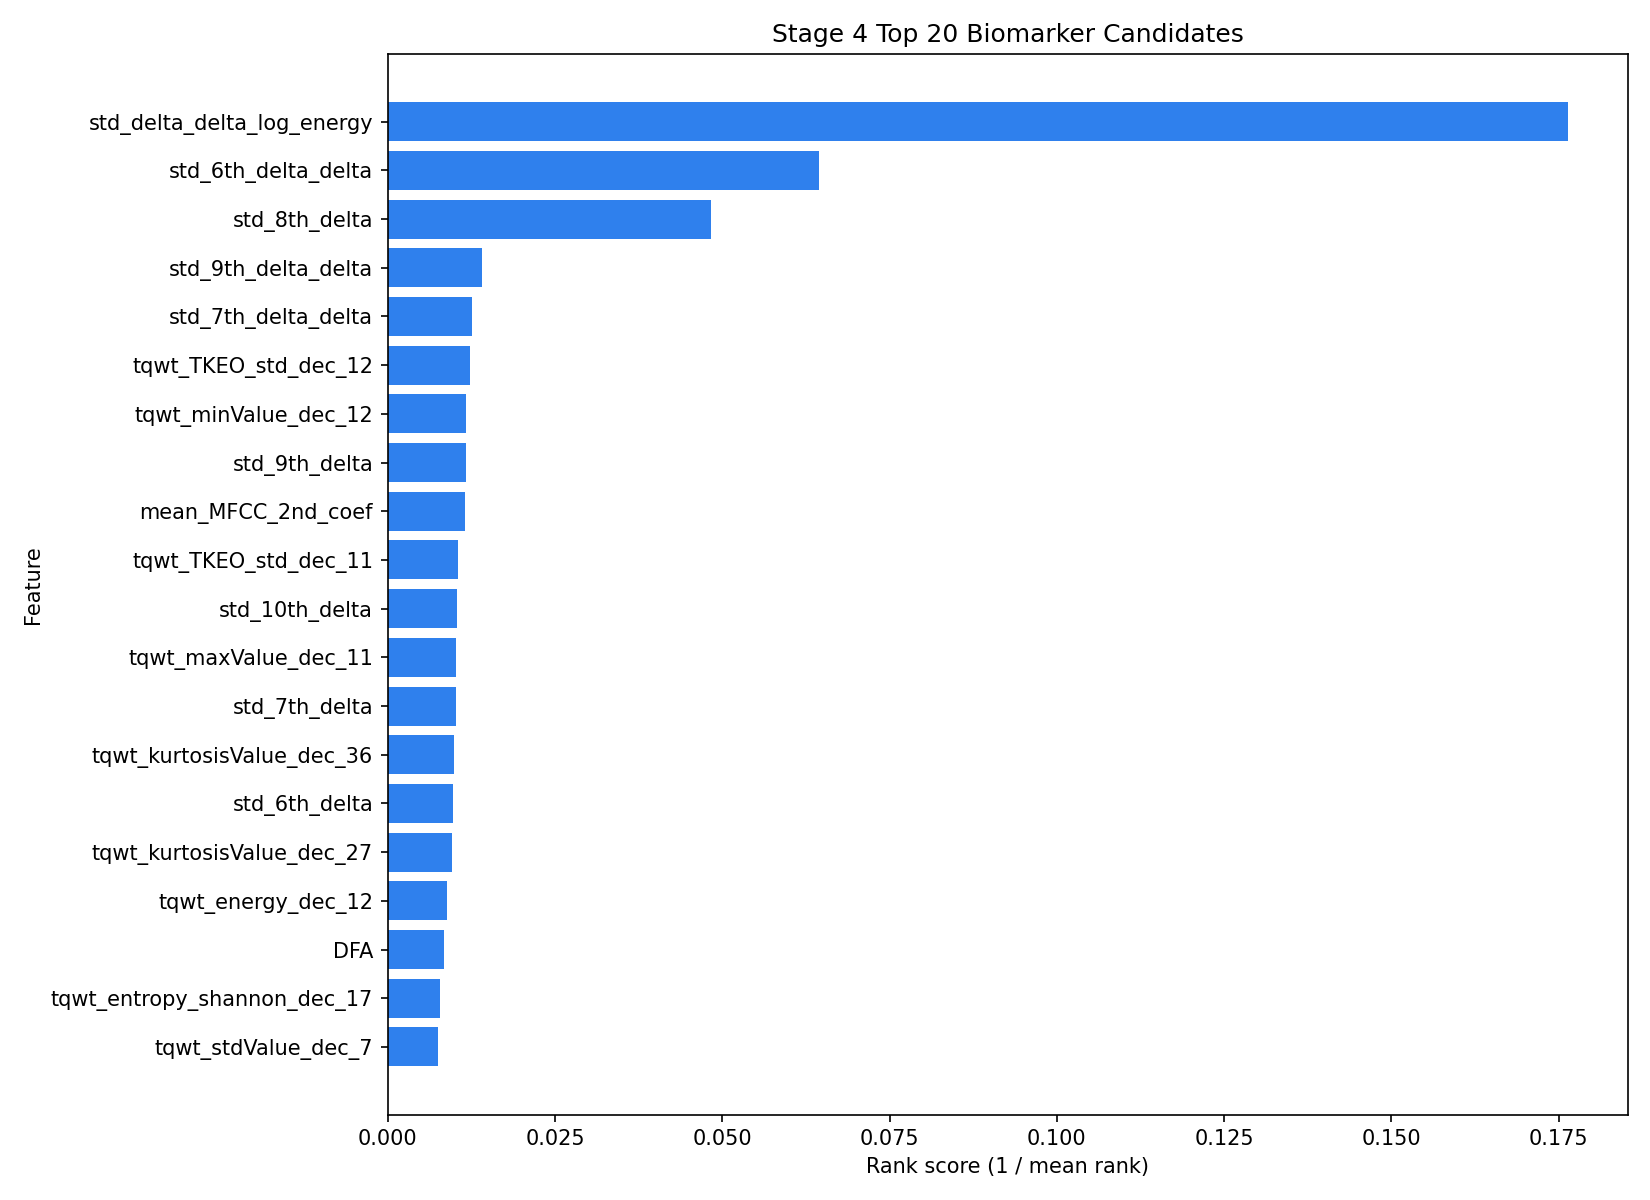
\includegraphics[width=0.86\textwidth]{figures/stage4_top20_biomarker_rank.png}
\caption{Top20 候选语音生物标志物综合排序}
\end{figure}

\begin{figure}[H]
\centering
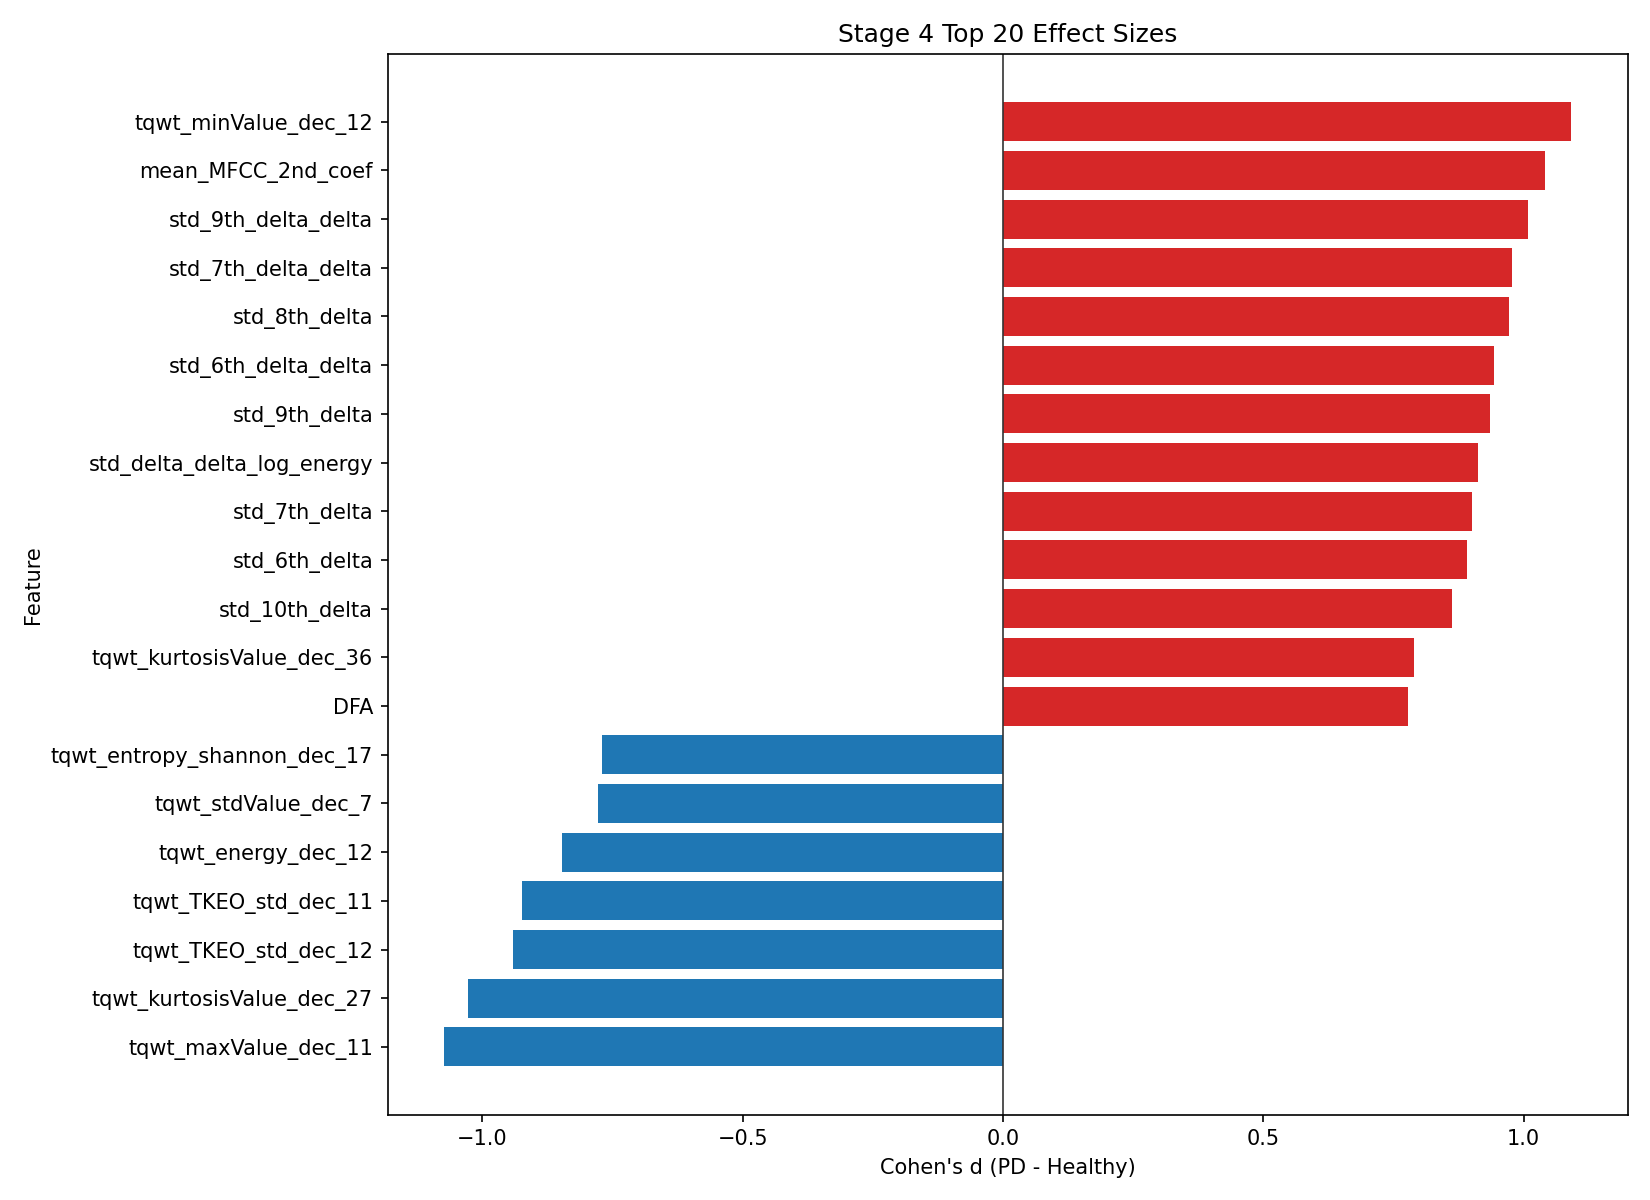
\includegraphics[width=0.86\textwidth]{figures/stage4_top20_effect_size.png}
\caption{Top20 候选特征效应量}
\end{figure}

\begin{figure}[H]
\centering
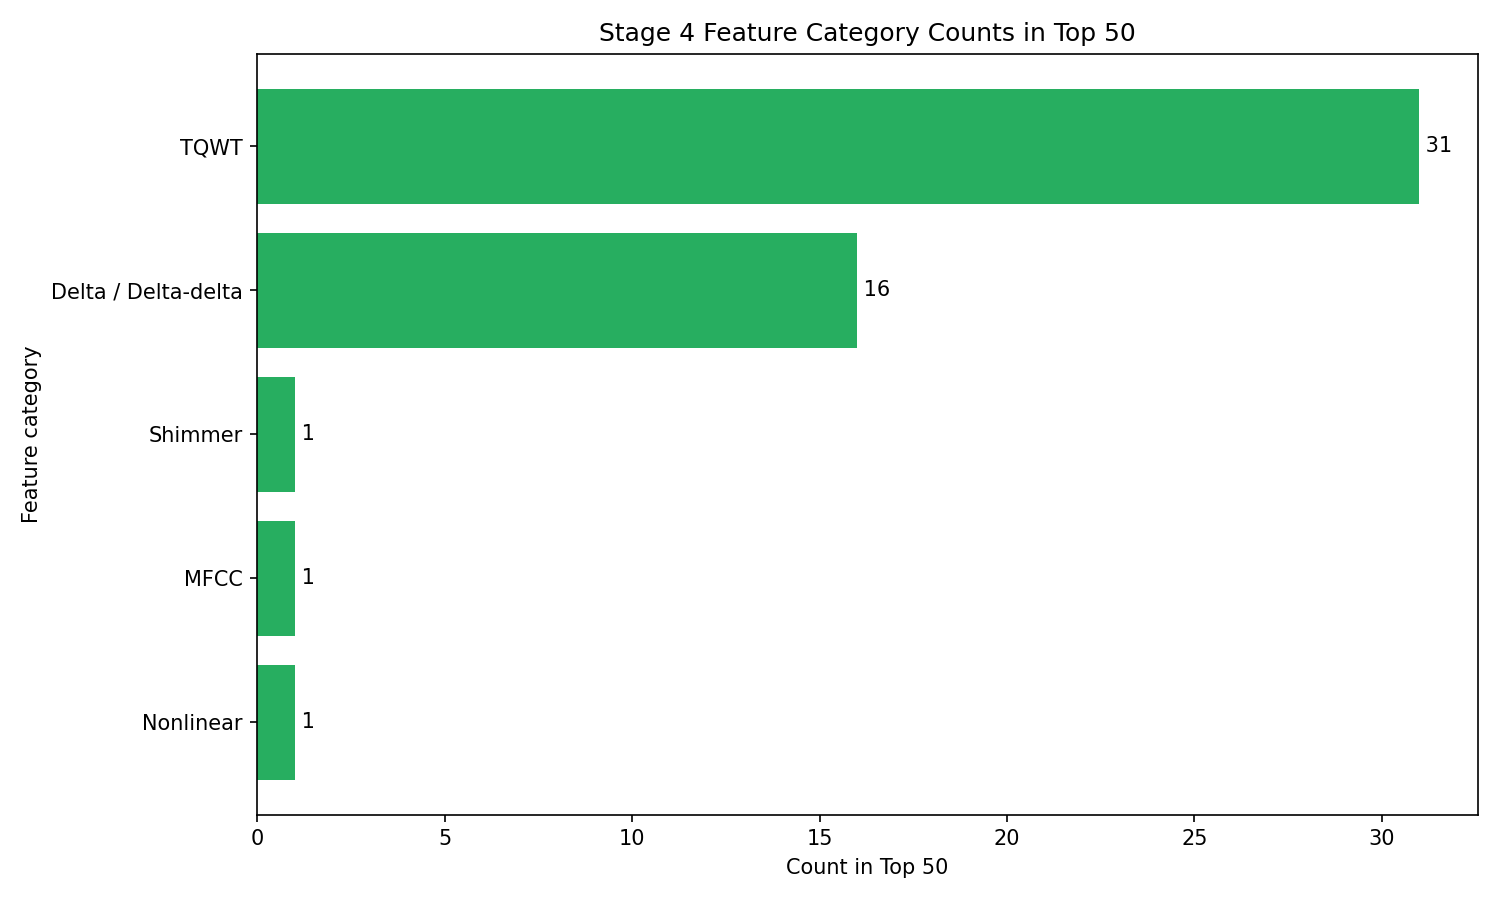
\includegraphics[width=0.72\textwidth]{figures/stage4_feature_category_counts_top50.png}
\caption{Top50 候选特征类别分布}
\end{figure}

上述特征只能称为候选语音生物标志物或判别性声学特征。由于本文没有临床机制实验和外部因果验证，不能作因果机制外推。

\clearpage
\section{模型三：Dataset 2 声音特征智能诊断}

Dataset 2 包含 80 名受试者、240 条录音，每名受试者 3 次录音，受试者级 Healthy 与 PD 各 40 名，类别均衡。该数据集的声学特征数为 44，与 Dataset 1 的高维 TQWT 特征空间不同，因此本文将其作为独立数据集单独建模和解释，而不与 Dataset 1 直接合并训练。

建模流程与模型一保持一致：输入为 acoustic-only 特征，主模型包括 Logistic Regression、SVM-RBF 和 Random Forest，并以 XGBoost 作为补充集成模型参考。交叉验证采用 StratifiedGroupKFold 并按 \feature{ID} 分组。标准化嵌入 Pipeline，仅在训练折内拟合。输出为受试者级 PD/Healthy 辅助诊断结果。

从表 2 可见，SVM-RBF 在 Dataset 2 上取得 accuracy 0.8375、balanced accuracy 0.8375、AUC 0.8906、sensitivity 0.8000、specificity 0.8750 和 F1 0.8300，综合表现最好。补充 XGBoost 的 accuracy 和 balanced accuracy 均为 0.7875，AUC 为 0.8563，未超过 SVM-RBF。Random Forest 的 specificity 较高但 sensitivity 较低，提示其对 Healthy 类更保守；Logistic Regression 的 sensitivity 较高但整体 accuracy 低于 SVM-RBF。

Dataset 2 样本量较小，但类别均衡、每名受试者录音次数一致，适合作为独立验证风格的参考分析。由于两个数据集特征空间不完全一致，本文不将 Dataset 2 结果解释为 Dataset 1 模型的严格外部验证，而作为同一研究问题下的独立声学诊断建模证据。

\clearpage
\section{模型四：二类潜在语音表型辅助分型}

\subsection{建模边界}

题目第四问涉及运动型和非运动型帕金森病，但给定数据没有真实运动型/非运动型临床标签。因此，本文不训练真实临床亚型监督分类器，而是在 Dataset 1 的 188 名 PD 受试者内部进行 \(k=2\) 无监督聚类，得到基于语音特征的二类潜在表型。该结果可作为探索性辅助分型线索，不能等同于真实临床亚型诊断。

\subsection{输入、方法与结果}

候选输入特征集包括 Top20、Top50、all acoustic 以及 PD-only 内部筛选得到的相关性去冗余、高 IQR/MAD 和 SparsePCA 表示方案。综合内部聚类指标、簇均衡性和 10000 组 Dirichlet 权重敏感性分析后，本文采用多候选报告口径。\feature{top20_biomarkers} / \feature{pca_5} / KMeans 的 top-1 频率最高，为 37.3\%，低于 60\% 的稳健主推荐阈值，因此表述为“相对推荐候选方案”，不作为唯一最优结论。

所有候选方案先执行标准化，再按方案进行 PCA 和聚类。聚类输入不包含 \feature{id}、\feature{gender}、\feature{class}、\feature{sex_male}、\feature{record_count} 或任何标签列。聚类质量通过 silhouette、Calinski-Harabasz、Davies-Bouldin 和重采样 ARI 等指标综合评价\upcite{silhouette,calinski,davies,ari}。

\begin{table}[H]
\centering
\caption{二类潜在语音表型相对推荐候选方案}
\begin{tabularx}{\textwidth}{lYccc}
\toprule
候选方案 & 特征 / 表示 / 聚类方法 & top-1 频率 & top-3 频率 & 判定 \\
\midrule
候选 1 & \feature{top20_biomarkers} / \feature{pca_5} / KMeans & 37.3\% & 63.2\% & 相对推荐 \\
候选 2 & \feature{top50_biomarkers} / \feature{pca_5} / KMeans & 22.4\% & 35.2\% & 可接受候选 \\
候选 3 & \feature{pd_high_iqr_top50} / \feature{pca_5} / AgglomerativeClustering & 21.0\% & 28.9\% & 可接受候选 \\
\bottomrule
\end{tabularx}
\end{table}

\begin{table}[H]
\centering
\caption{二类潜在语音表型相对推荐方案指标}
\begin{tabularx}{\textwidth}{lY}
\toprule
项目 & 数值 \\
\midrule
相对推荐候选方案 & \feature{top20_biomarkers} / \feature{pca_5} / KMeans \\
PD 受试者数 & 188 \\
Cluster 0 人数 & 62 \\
Cluster 1 人数 & 126 \\
Smaller cluster ratio & 0.3298 \\
Silhouette & 0.3674 \\
Stability ARI mean & 0.9897 \\
权重敏感性 top-1 频率 & 37.3\% \\
\bottomrule
\end{tabularx}
\end{table}

\begin{figure}[H]
\centering
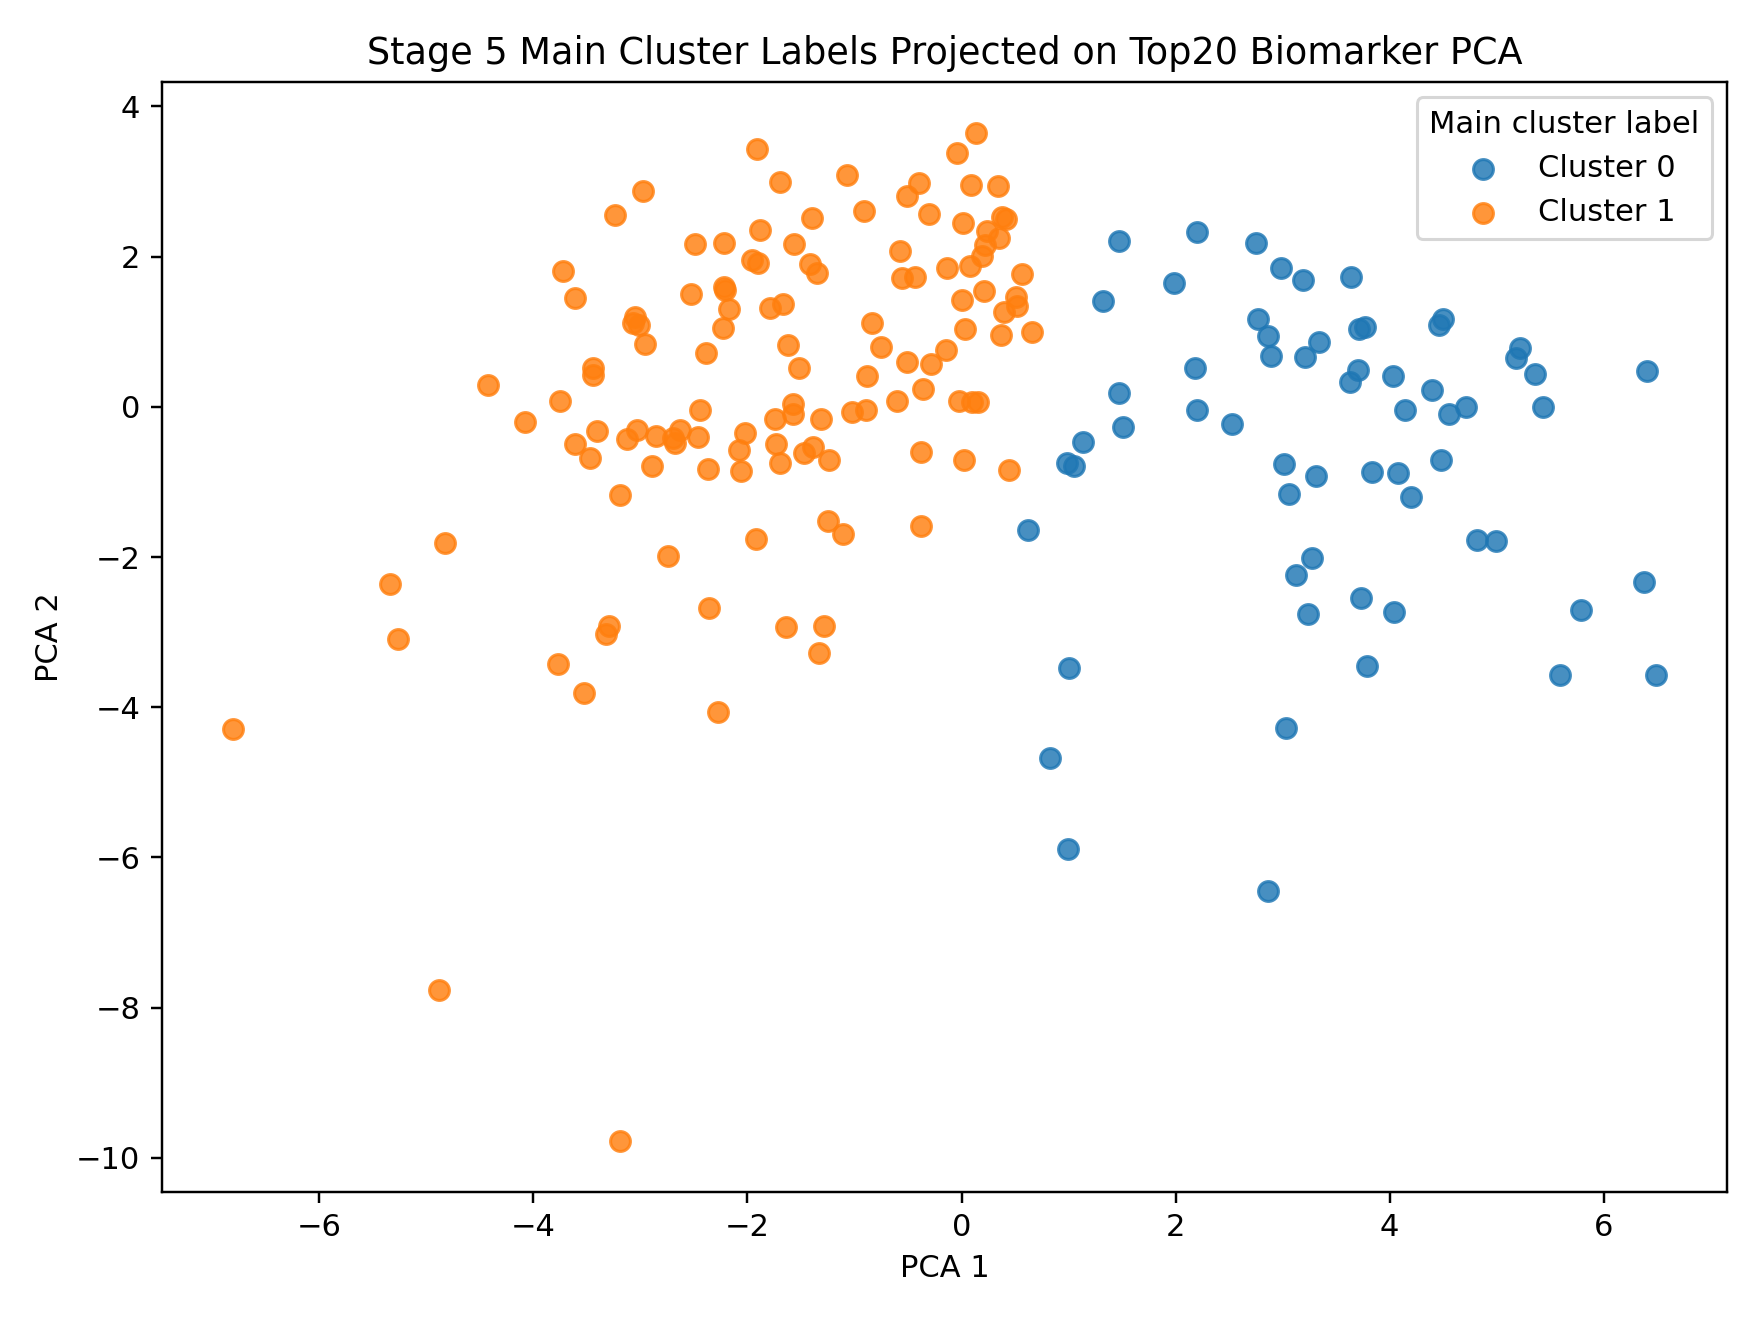
\includegraphics[width=0.82\textwidth]{figures/stage5_pca_k2_clusters_top20.png}
\caption{Dataset 1 PD 受试者二类潜在语音表型 PCA 可视化}
\end{figure}

该图将相对推荐候选方案得到的二类聚类标签投影到 Top20 特征的前两个 PCA 方向上。图中两类样本在二维空间中呈现较明显的左右分离趋势，说明 Top20 候选特征能够支持 PD 受试者内部的二类潜在语音表型划分。但 PCA 二维图只是可视化投影，不能替代 silhouette、簇规模和稳定性 ARI 等定量指标，也不能直接说明真实临床亚型存在。

\begin{figure}[H]
\centering
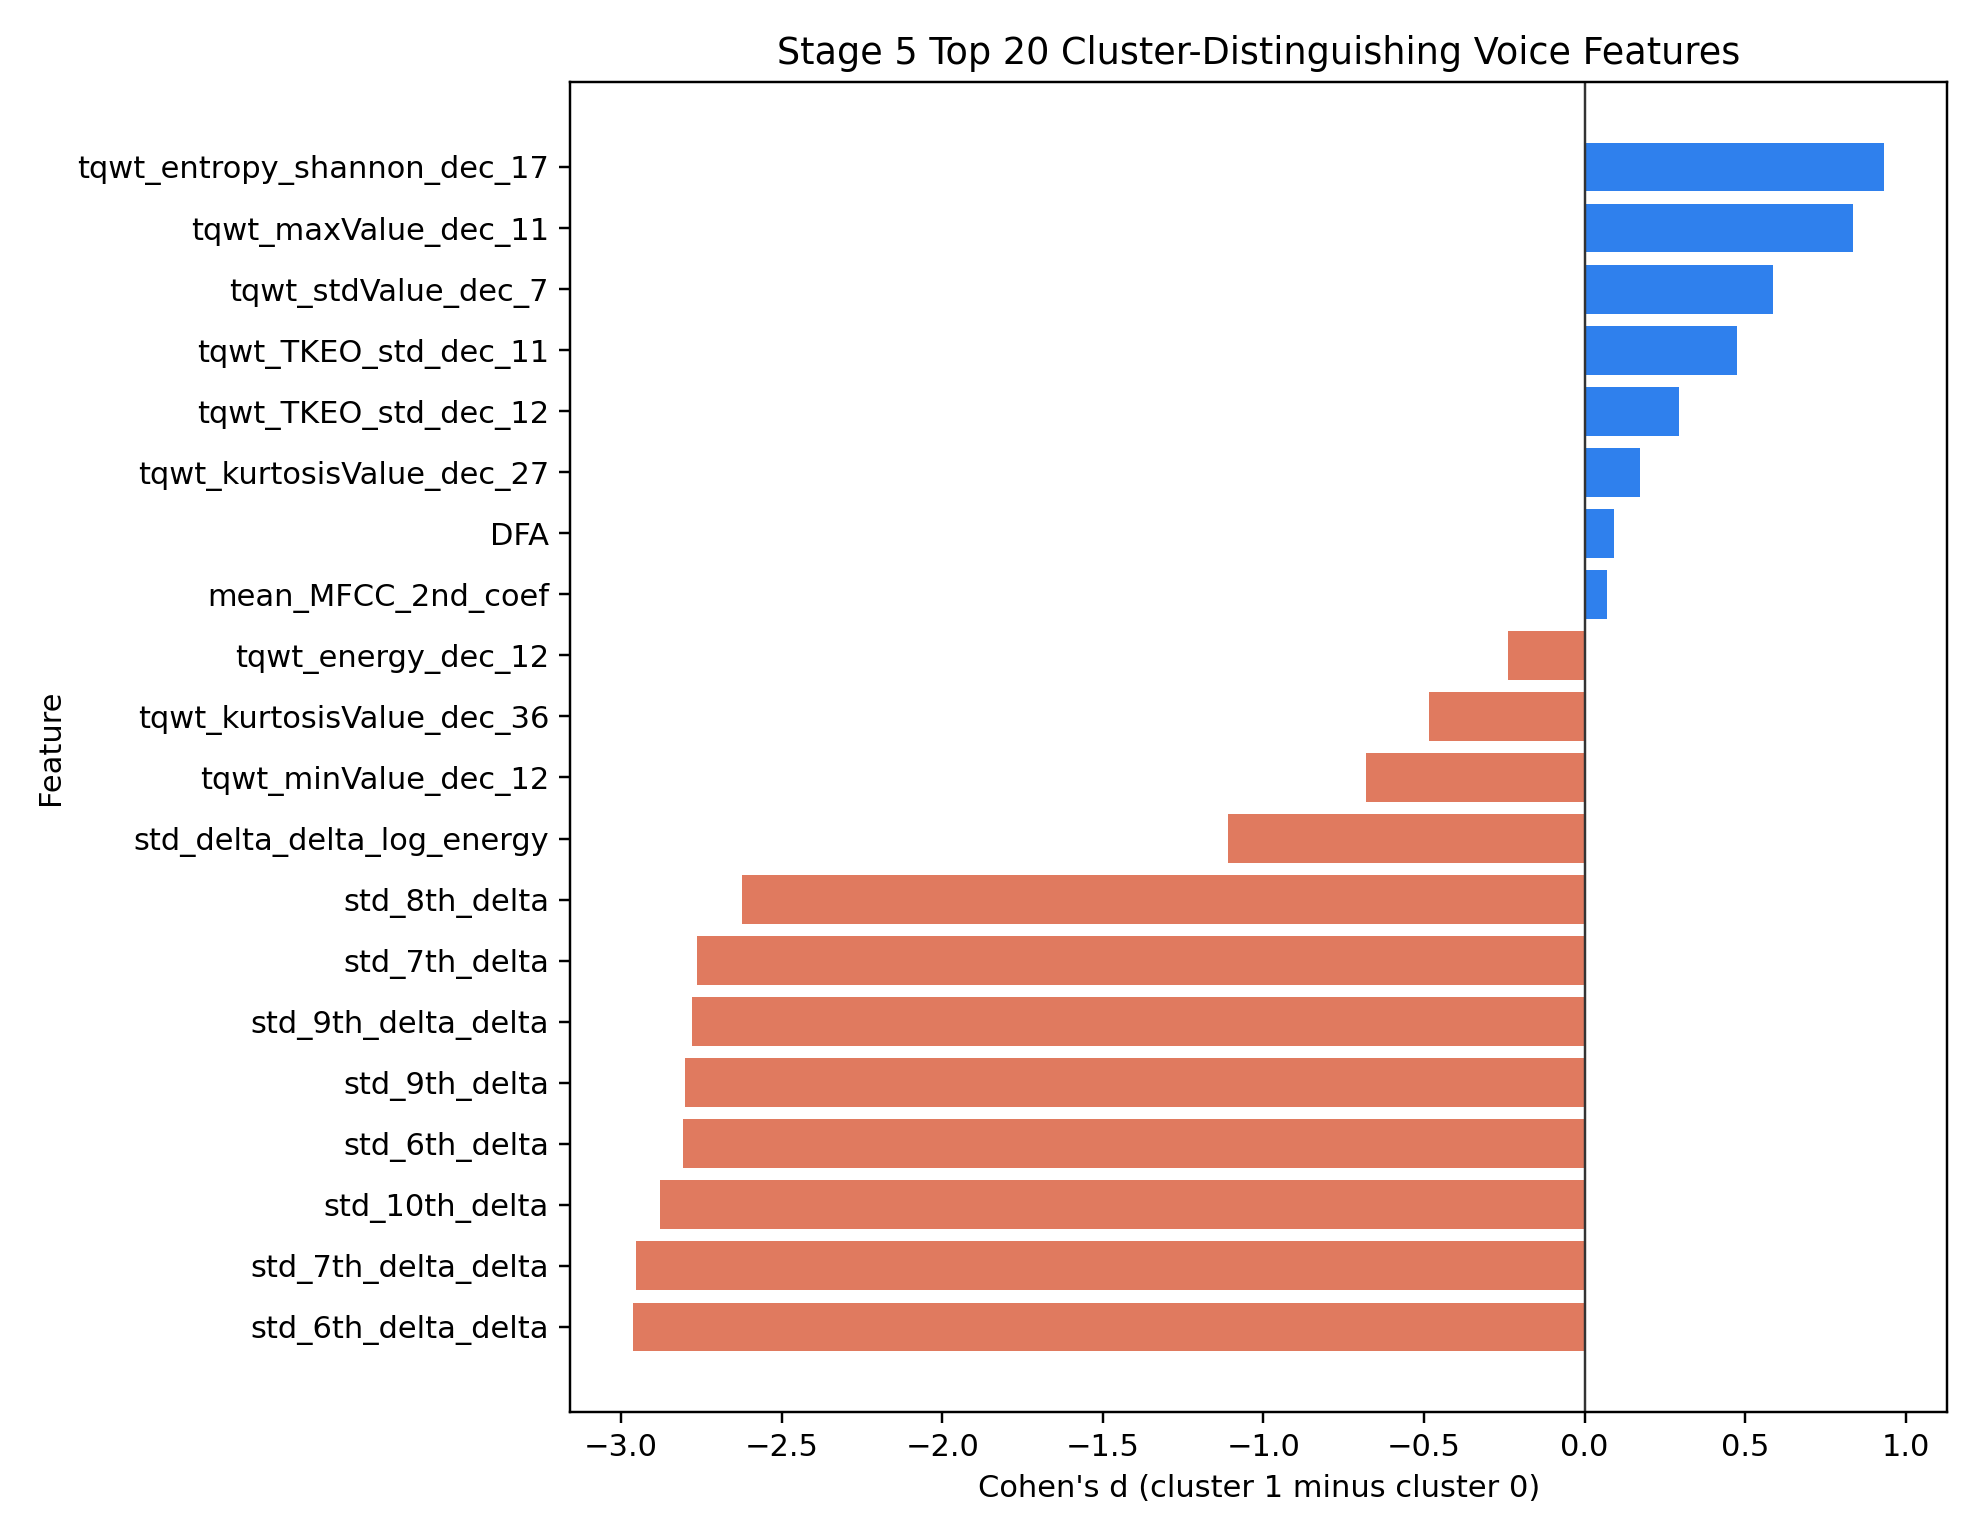
\includegraphics[width=0.88\textwidth]{figures/stage5_cluster_feature_difference_top20.png}
\caption{二类潜在语音表型的 Top20 特征差异}
\end{figure}

该图以 Cohen's \(d\) 展示二类潜在表型在 Top20 特征上的差异方向。横轴为 cluster 1 minus cluster 0，因此负值表示 cluster 0 更高，正值表示 cluster 1 更高。图中 cluster 0 在多项 Delta / Delta-delta 动态谱波动特征上更高，cluster 1 在若干 TQWT 特征上更高，提示两簇主要反映动态谱波动和多尺度声学结构的差异。该差异只能解释为语音表型差异，不能直接解释为真实运动型/非运动型临床差异。

\subsection{表型解释}

相对推荐候选方案得到 cluster 0 共 62 人、cluster 1 共 126 人。cluster 0 在多项 Delta / Delta-delta 动态谱波动特征上更高，例如 \feature{std_6th_delta_delta}、\feature{std_7th_delta_delta}、\feature{std_10th_delta}、\feature{std_6th_delta} 等。cluster 1 在部分 TQWT 多尺度特征上更高，例如 \feature{tqwt_entropy_shannon_dec_17}、\feature{tqwt_maxValue_dec_11}、\feature{tqwt_stdValue_dec_7}、\feature{tqwt_TKEO_std_dec_11} 等。

后续聚类标签复现模型学习的是上述无监督聚类标签，用于将探索性分型规则模型化。该分类器不是根据真实运动型/非运动型标签训练，不能解释为真实临床亚型诊断性能。

\clearpage
\section{模型五：六类潜在语音表型辅助分型}

\subsection{建模边界}

题目第五问涉及六类帕金森病症状，但数据集中没有静止性震颤、运动迟缓、肌肉僵直、疼痛、痴呆、睡眠障碍六类真实临床症状标签。因此，本文只在 Dataset 1 的 188 名 PD 受试者内部固定 \(k=6\) 进行无监督聚类，输出基于语音特征的六类潜在表型。六个 cluster 编号没有直接临床症状含义，仍需真实临床症状标签进一步验证。

\subsection{输入、方法与结果}

六类表型建模对 Top20、Top50 和 all acoustic 特征集进行候选方案比较，并做 \(k=2\) 到 \(k=8\) 的参考扫描。主方案为 \feature{top20_biomarkers} / \feature{pca_5} / AgglomerativeClustering。所有表示均先进行标准化，PCA 和聚类仅使用声学特征；二类聚类标签没有进入六类聚类输入。

\begin{table}[H]
\centering
\caption{六类潜在语音表型主方案指标}
\begin{tabularx}{\textwidth}{lY}
\toprule
项目 & 数值 \\
\midrule
主方案 & \feature{top20_biomarkers} / \feature{pca_5} / AgglomerativeClustering \\
PD 受试者数 & 188 \\
六簇人数 & 13、55、34、28、25、33 \\
最小簇比例 & 0.0691 \\
Silhouette & 0.1823 \\
Stability ARI mean & 0.4582 \\
二类与六类表型 NMI & 0.4089 \\
Collapsed majority ARI & 0.8128 \\
\bottomrule
\end{tabularx}
\end{table}

\begin{figure}[H]
\centering
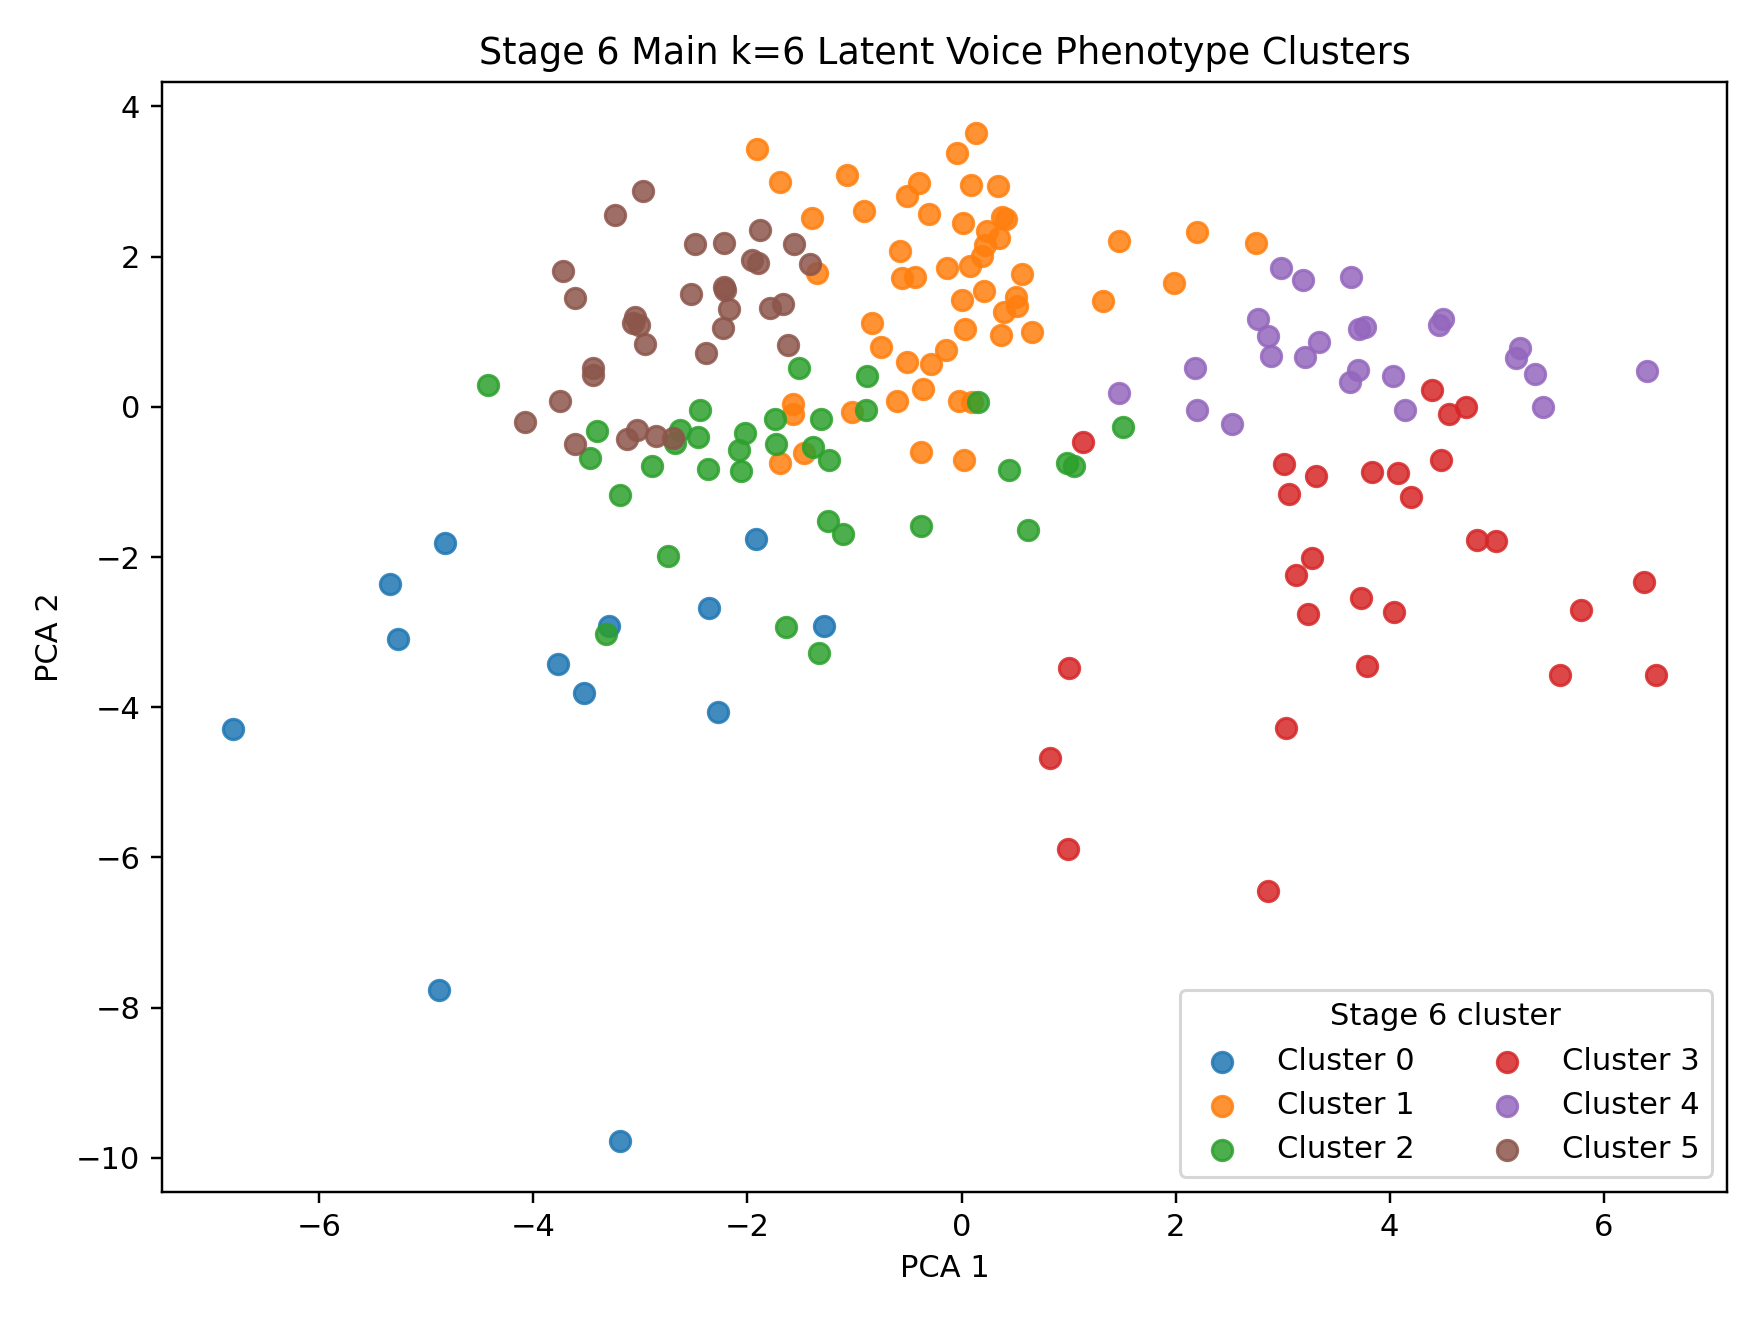
\includegraphics[width=0.84\textwidth]{figures/stage6_pca_k6_clusters_main.png}
\caption{Dataset 1 PD 受试者六类潜在语音表型 PCA 可视化}
\end{figure}

\begin{figure}[H]
\centering
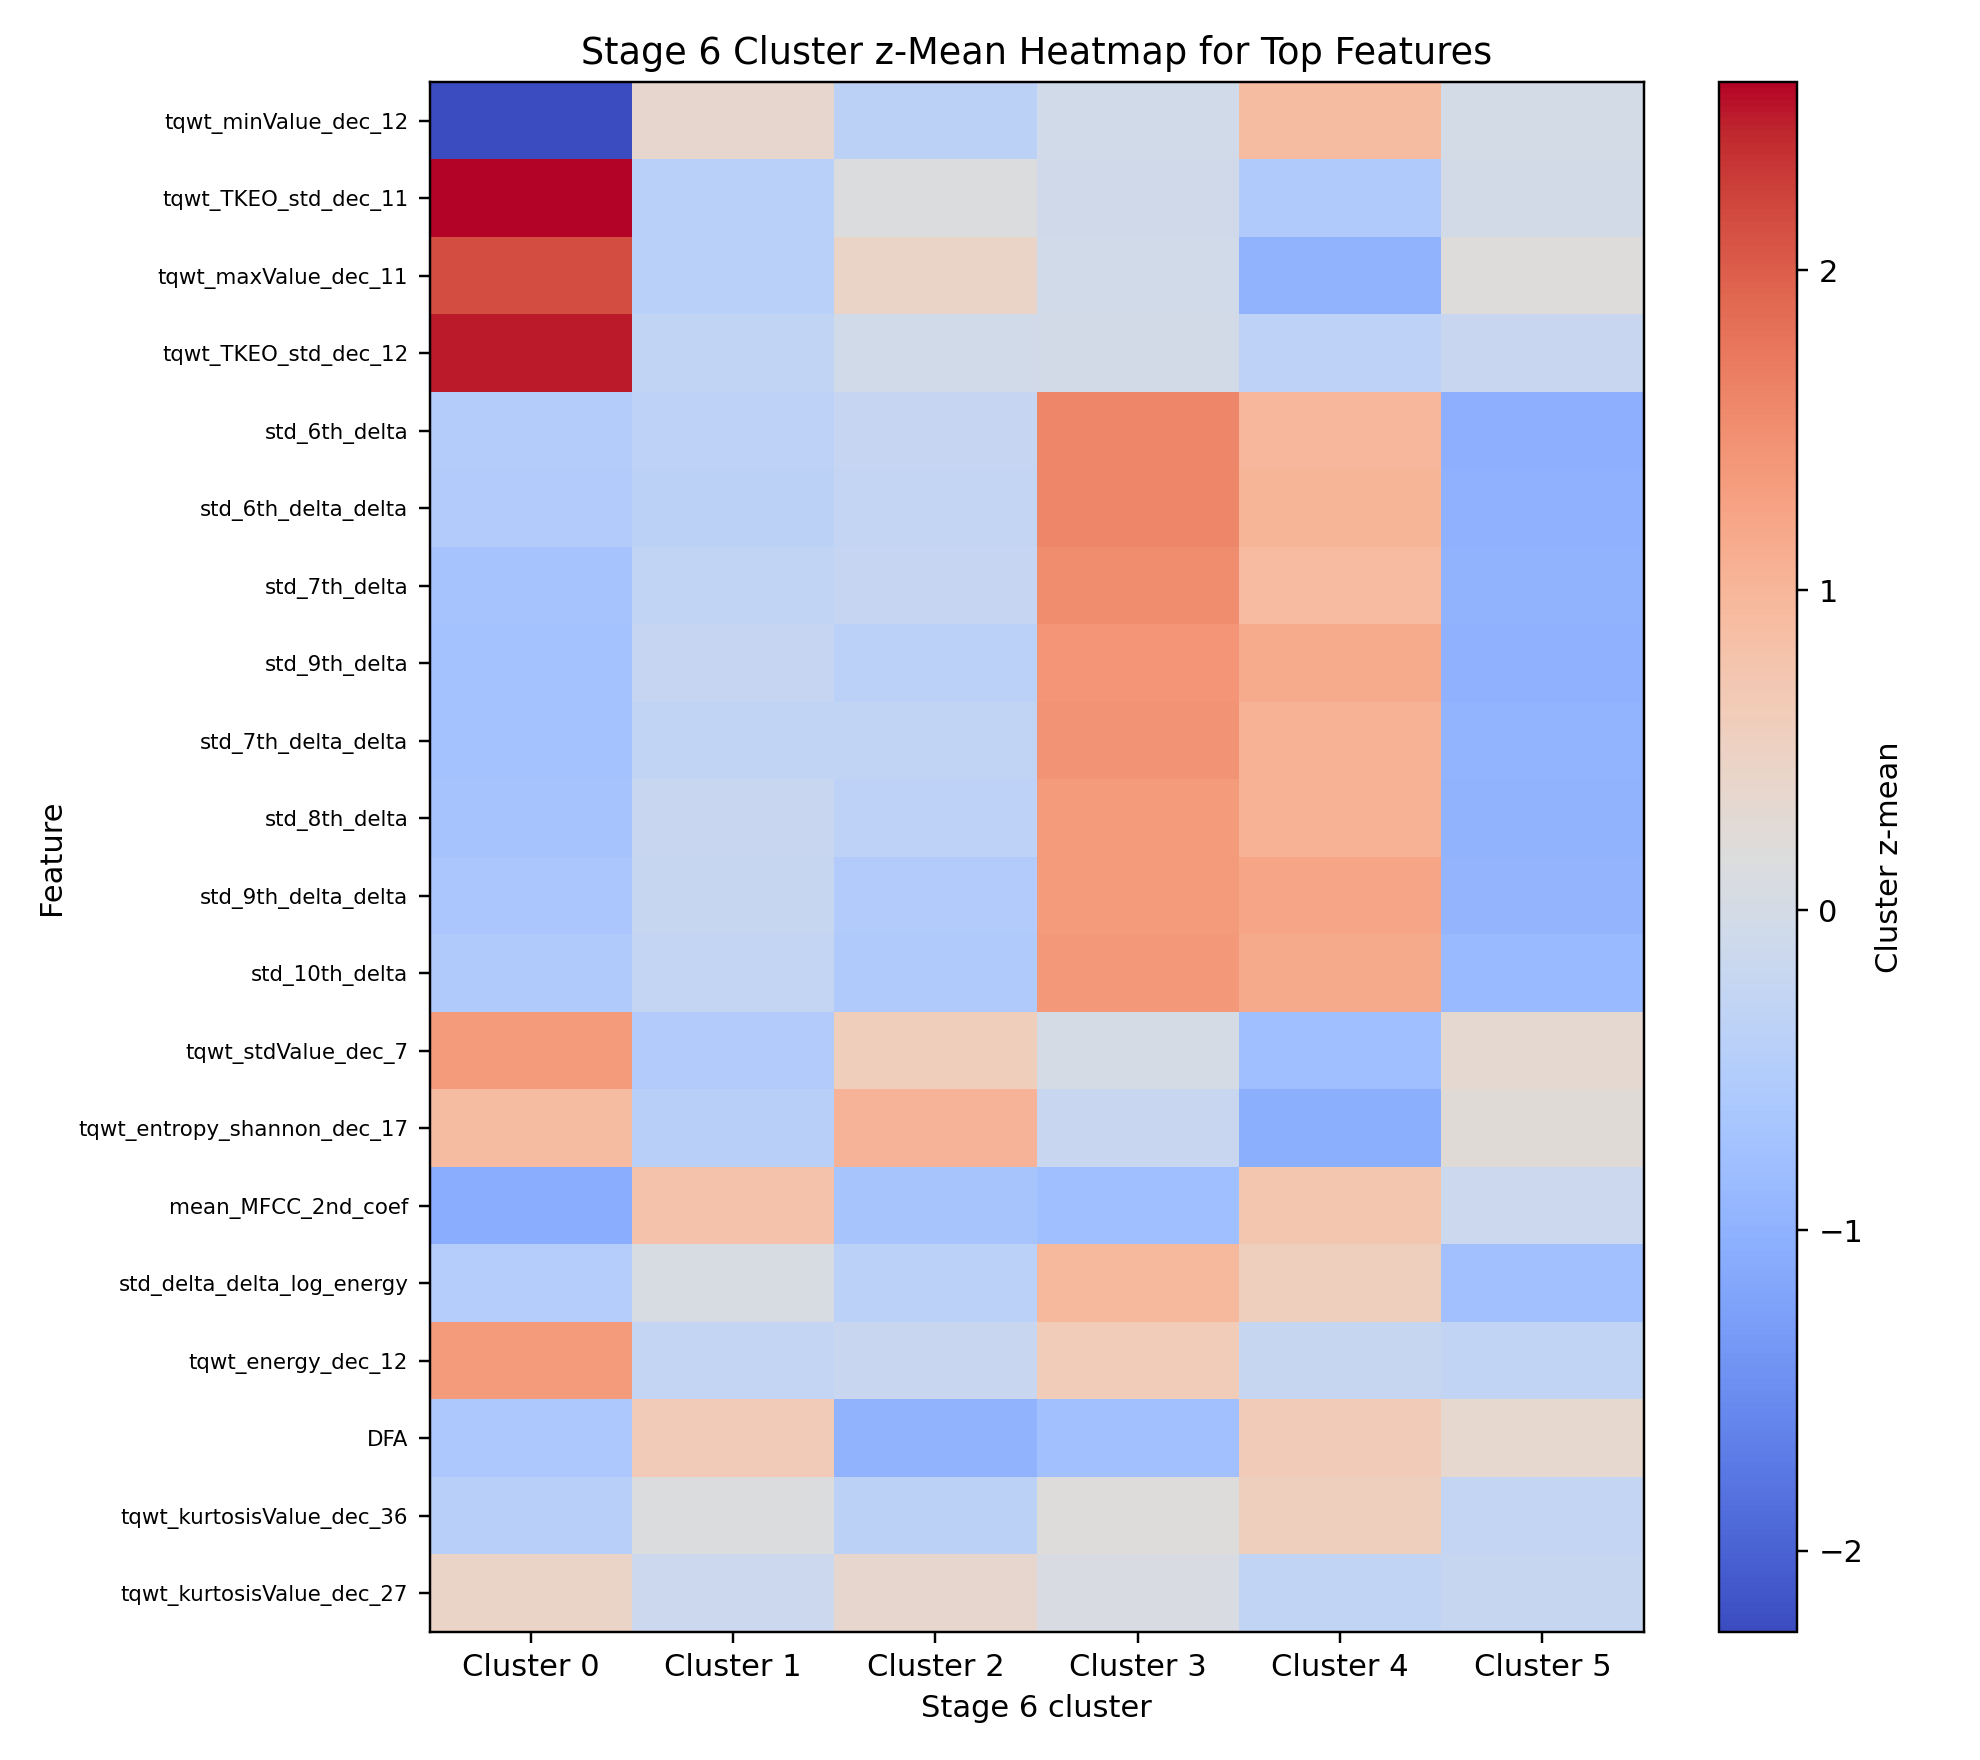
\includegraphics[width=0.9\textwidth]{figures/stage6_cluster_feature_heatmap.png}
\caption{六类潜在语音表型特征热图}
\end{figure}

\begin{figure}[H]
\centering
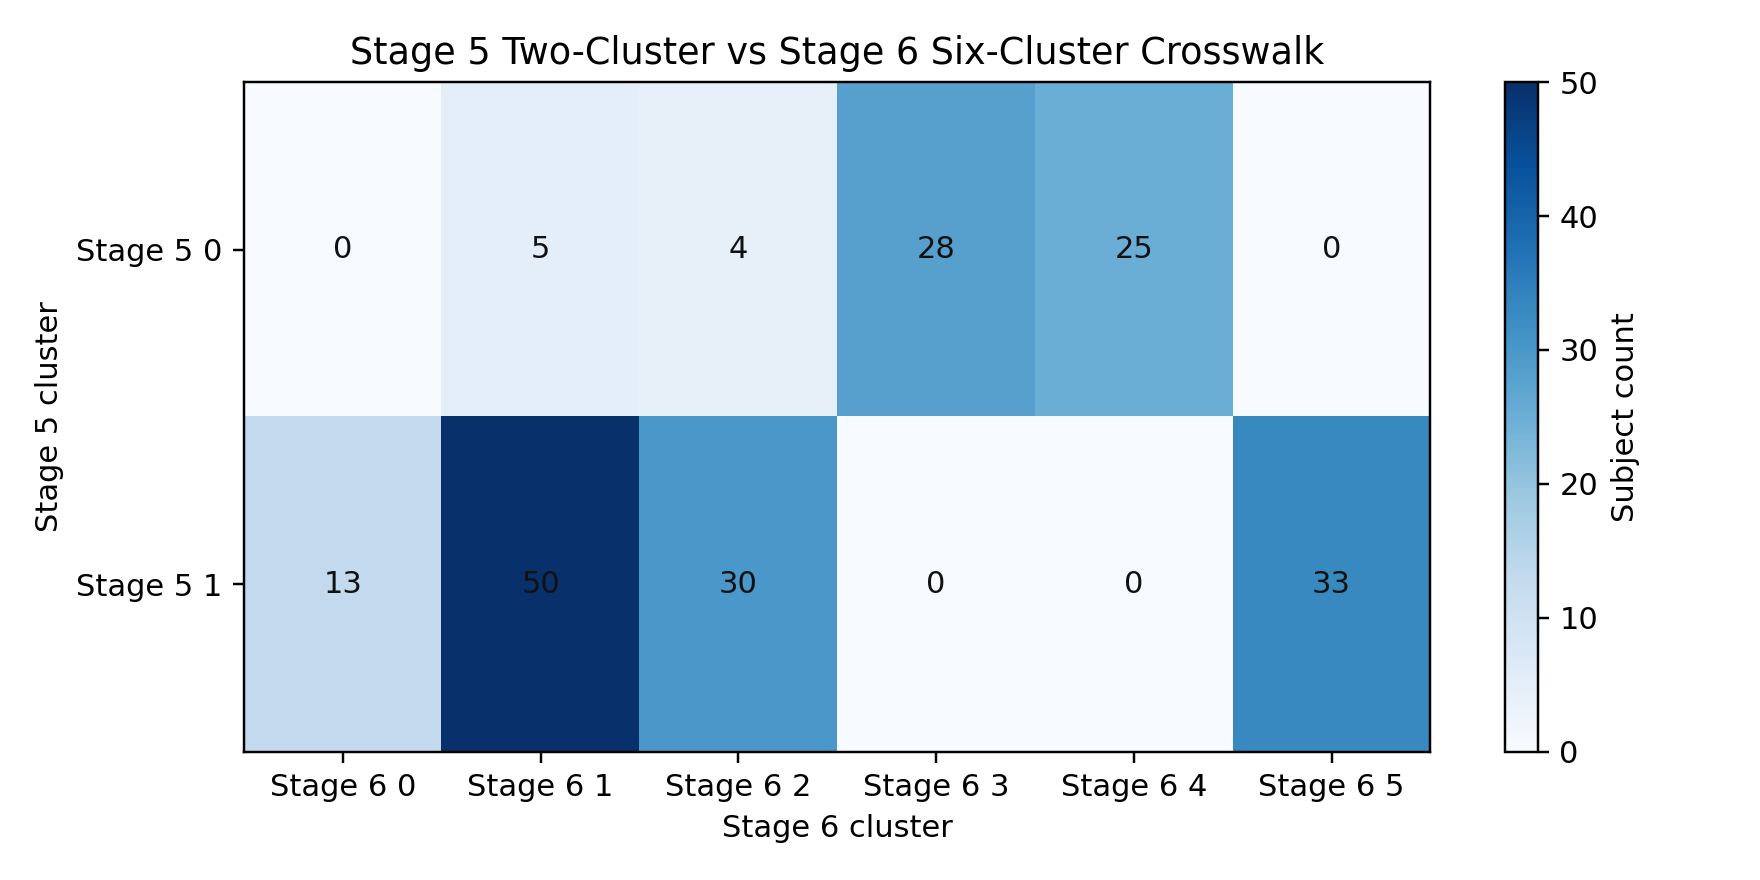
\includegraphics[width=0.76\textwidth]{figures/stage6_stage5_crosswalk_heatmap.png}
\caption{二类潜在表型与六类潜在表型交叉关系}
\end{figure}

\subsection{结果解释}

六类潜在语音表型主要由 Delta / Delta-delta 与 TQWT 特征区分。部分簇表现为动态谱波动特征较高，部分簇则表现为 TQWT 多尺度能量、熵或统计量差异。与二类方案相比，六类方案的 silhouette 下降到 0.1823，stability ARI mean 下降到 0.4582，说明固定 \(k=6\) 后聚类结构更细但稳定性和分离度较弱。

六类潜在表型与二类潜在表型存在一定嵌套关系，NMI 为 0.4089，按六簇多数映射回二簇后的 collapsed majority ARI 为 0.8128。该交叉关系只能说明六类潜在表型与二类潜在表型在声学空间中存在一定对应，不能解释为真实临床分层诊断。

六类聚类标签复现模型预测的是六类聚类标签，不是真实静止性震颤、运动迟缓、肌肉僵直、疼痛、痴呆或睡眠障碍标签。因此，其指标只表示复现无监督聚类划分的能力，不表示六类临床症状诊断能力。

\clearpage
\section{模型优缺点分析}

\subsection{优点}

第一，本文严格识别了两个数据集的重复录音结构，监督学习中按受试者分组交叉验证，并以 subject-level 指标作为主结果，降低了样本单位错误带来的性能高估风险。第二，主声学模型排除了 \feature{sex_male}，避免将人口学变量混入声学诊断结论。第三，候选语音生物标志物识别同时结合统计检验、效应量、稳定选择和模型重要性，并以 XGBoost/SHAP 作补充解释一致性检查，使特征解释不依赖单一方法。第四，对缺少真实标签的第四问和第五问，本文采用无监督潜在表型分析，并明确其探索性边界。第五，全流程一致性检查对分组、泄漏和指标一致性进行了系统控制。

\subsection{局限性}

本文也存在明显局限。Dataset 1 受试者数有限且类别不均衡，导致部分模型特异度偏低；补充 XGBoost 虽提高了部分判别指标，但同样表现出 specificity 偏低的问题，不能据此写成临床确诊模型。Dataset 2 虽类别均衡，但样本量较小。两个数据集的特征空间不完全一致，不能简单合并或直接外推。SHAP 解释反映的是模型预测贡献，不等同于临床因果机制。第四问和第五问缺少真实临床症状标签，因此聚类结果只能称为潜在语音表型，不能直接对应运动型/非运动型或六类临床症状。聚类表型仍需要真实临床标签、纵向随访和外部样本验证。

\clearpage
\section{结论}

针对问题一，Dataset 1 的 PD/Healthy 辅助诊断模型表明，语音声学特征具有一定判别能力。Random Forest 的 accuracy 和 AUC 较高，但 specificity 较低，提示其偏向 PD 类；SVM-RBF 在 balanced accuracy 上表现相对稳健。

针对问题二，综合多种统计和模型解释证据，本文得到 Top20 候选语音生物标志物。其中特征主要集中于 Delta / Delta-delta 动态谱波动和 TQWT 多尺度声学结构，说明这些声学维度对 PD/Healthy 判别具有较强关联性，但不能解释为临床因果结论。

针对问题三，Dataset 2 按受试者 ID 分组交叉验证后，SVM-RBF 取得 accuracy 0.8375、balanced accuracy 0.8375 和 AUC 0.8906，是该数据集上的主推荐模型。该结论支持语音特征在独立数据集中的辅助诊断价值，但仍受样本量限制。

针对问题四，本文在 188 名 PD 受试者内部得到二类潜在语音表型。主方案 silhouette 为 0.3674，stability ARI mean 为 0.9854，显示较稳定的二类声学结构。该结构主要由动态谱波动特征和部分 TQWT 特征区分，但不是真实运动型/非运动型诊断。

针对问题五，本文固定 \(k=6\) 得到六类潜在语音表型。六簇主要由 Delta / Delta-delta 与 TQWT 特征区分，但其 silhouette 和稳定性弱于二类方案，因此只能作为探索性六类语音表型。后续若获得真实六类临床症状标签，应重新建立受试者级监督验证框架。

总体而言，语音声学特征对帕金森病辅助筛查、判别性特征识别和探索性分型具有应用潜力。本文结论应定位为辅助建模证据和探索性语音表型分析，而非临床确诊模型。

\clearpage
\begin{thebibliography}{99}

\bibitem{dataset1}
Sakar B E, Isenkul M E, Sakar C O, et al. Collection and analysis of a Parkinson speech dataset with multiple types of sound recordings[J]. IEEE Journal of Biomedical and Health Informatics, 2013, 17(4): 828--834.

\bibitem{dataset2}
Naranjo L, Perez C J, Campos-Roca Y, Martin J. Addressing voice recording replications for Parkinson's disease detection[J]. Expert Systems with Applications, 2016, 46: 286--292.

\bibitem{review}
A review of machine learning and deep learning for Parkinson's disease[C/OL]. 见 \feature{problem/A review of machine learning and deep learning for Parkinson's.pdf}. % TODO: 核对文献信息

\bibitem{sklearn}
Pedregosa F, Varoquaux G, Gramfort A, et al. Scikit-learn: Machine learning in Python[J]. Journal of Machine Learning Research, 2011, 12: 2825--2830.

\bibitem{benjamini}
Benjamini Y, Hochberg Y. Controlling the false discovery rate: a practical and powerful approach to multiple testing[J]. Journal of the Royal Statistical Society: Series B, 1995, 57(1): 289--300.

\end{thebibliography}

\clearpage
\appendix
\section{附录：程序代码}

本附录给出建模、特征识别、潜在表型分析与权重敏感性分析所用的完整代码。XGBoost 补充二分类模型位于代码二，XGBoost 特征重要性与 SHAP 解释性分析位于代码三。为避免正文被程序实现细节打断，代码统一置于附录。

\subsection{代码一：数据预处理与质量控制}
\VerbatimInput[fontsize=\tiny,breaklines=true,breakanywhere=true,numbers=left,numbersep=4pt,xleftmargin=1.8em]{../src/stage2_qc_pipeline.py}

\clearpage
\subsection{代码二：二分类辅助诊断模型与 XGBoost 补充模型}
\VerbatimInput[fontsize=\tiny,breaklines=true,breakanywhere=true,numbers=left,numbersep=4pt,xleftmargin=1.8em]{../src/stage3_baseline_models.py}

\clearpage
\subsection{代码三：判别性声学特征识别与 XGBoost/SHAP 解释性分析}
\VerbatimInput[fontsize=\tiny,breaklines=true,breakanywhere=true,numbers=left,numbersep=4pt,xleftmargin=1.8em]{../src/stage4_biomarker_identification.py}

\clearpage
\subsection{代码四：二类潜在语音表型建模}
\VerbatimInput[fontsize=\tiny,breaklines=true,breakanywhere=true,numbers=left,numbersep=4pt,xleftmargin=1.8em]{../src/stage5_pd_two_cluster_phenotyping.py}

\clearpage
\subsection{代码五：六类潜在语音表型建模}
\VerbatimInput[fontsize=\tiny,breaklines=true,breakanywhere=true,numbers=left,numbersep=4pt,xleftmargin=1.8em]{../src/stage6_pd_six_cluster_phenotyping.py}

\clearpage
\subsection{代码六：PD 内部分型特征扩展与权重敏感性分析}
\VerbatimInput[fontsize=\tiny,breaklines=true,breakanywhere=true,numbers=left,numbersep=4pt,xleftmargin=1.8em]{../src/stage5b_stage6b_pdonly_sensitivity.py}


\end{document}
